\newpage
\section{Umsetzung}
Dieses Kapitel befasst sich mit der Umsetzung des ausgearbeiteten Konzepts aus Kapitel XY. Dabei sind die Unterkapitel nach Funktion geordnet.

\subsection{Überblick}
Zur Förderung des besseren Verständnis wird das umgesetzte Gesamtkonzept kurz vorgestellt.  Der Pflanzroboter bildet eine Einheit, bestehend aus:
	\begin{figure}[H]
	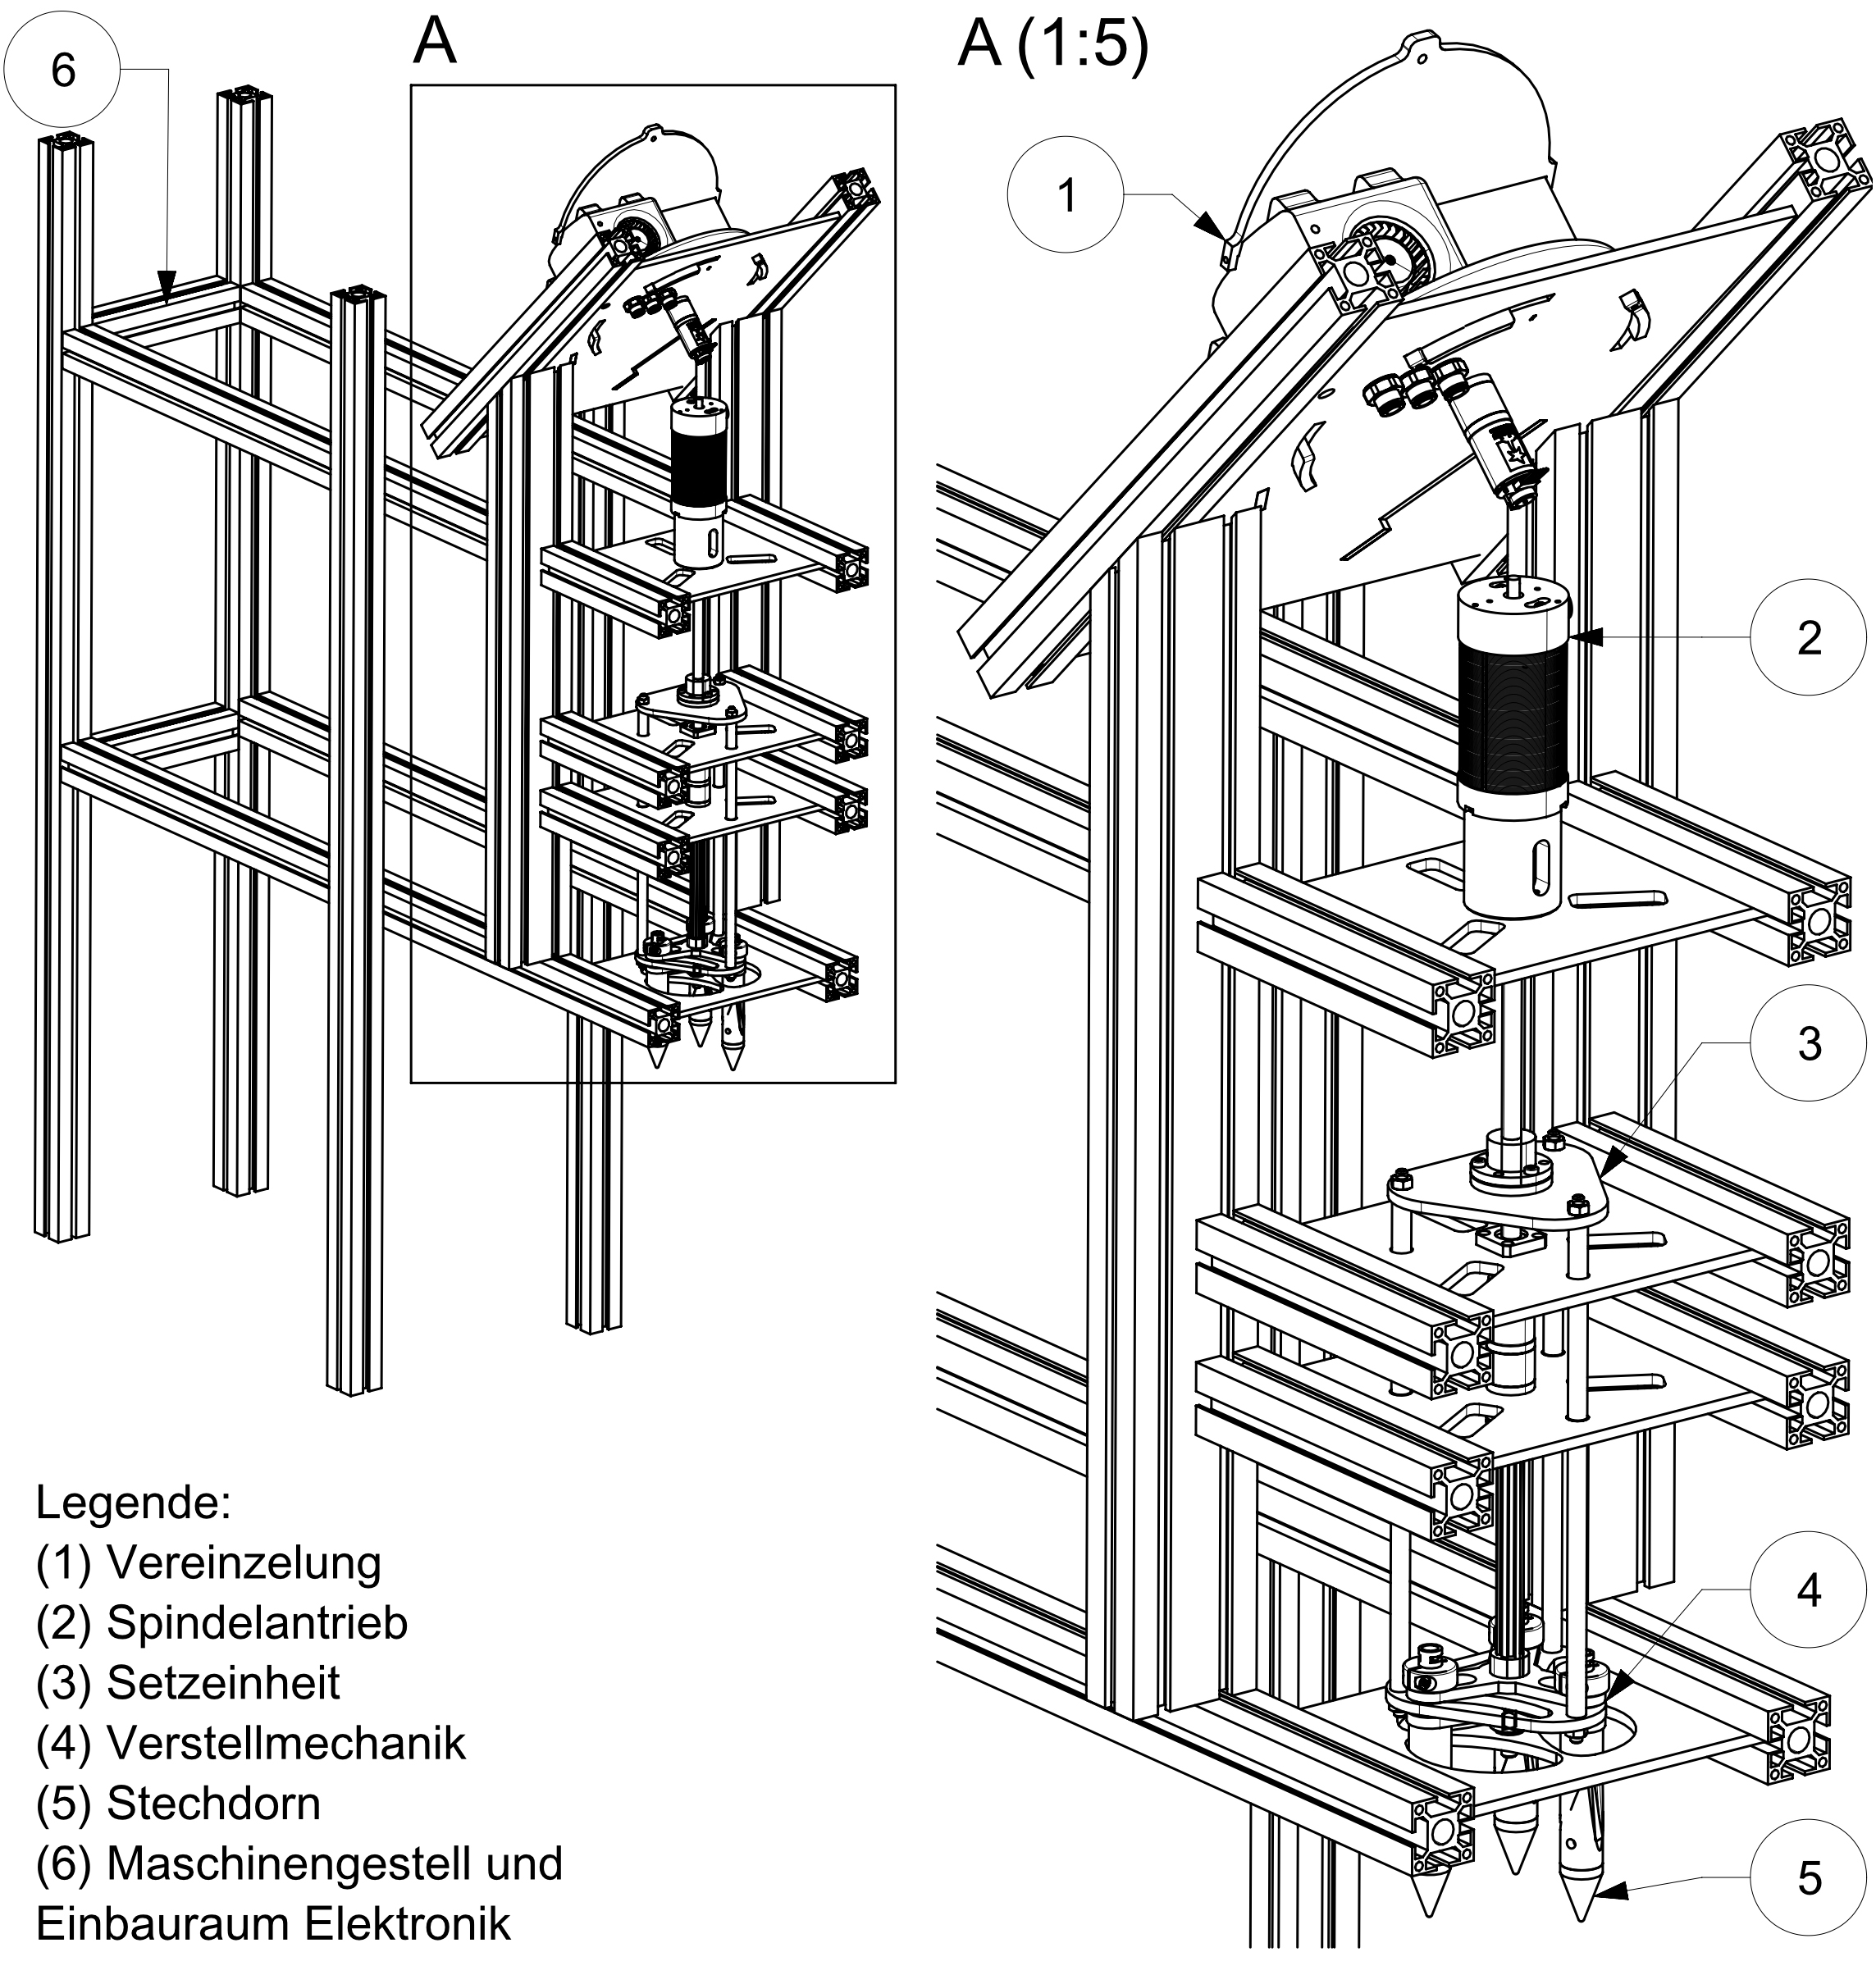
\includegraphics[scale=0.55]{Illustrationen/6-Umsetzung/uberblick.png}
	\caption{Perspektivische Ansicht des Pflanzroboter}
	\label{fig:uberblick}
	\end{figure}
Konstruktiv konnten die Schläuche, welche die Vereinzelung mit dem Stechdornen verbindet, nicht in der Abbildung \ref{fig:uberblick} nicht dargestellt werden. Auch das Maschinengestell inklusive Einbauraum für die Elektronik ist unvollständig abgebildet. Der zeichnerische Aufwand steht nicht im Verhältnis zum Nutzen und würde den Zeitrahmen der Bachelorarbeit überschreiten. 
